\documentclass[12pt,a4paper]{article}
\usepackage[utf8]{inputenc}
\usepackage[T1]{fontenc}
\usepackage[english]{babel}
\usepackage{fancyhdr}
\usepackage{kpfonts}
\usepackage[margin=1in]{geometry}
\usepackage{exsheets}
\usepackage{amsmath, amssymb, amsfonts}
\usepackage{enumerate}
\usepackage{tikz}
\usetikzlibrary{arrows, decorations.text}

\pagestyle{fancy}
\renewcommand{\headrulewidth}{2pt}
\fancyhead[L]{EPITA\_ING1\_BING\_2018\_S6\_PARTIEL\_GREF}
\fancyhead[R]{June 2017}

\fancyfoot[C]{\textbf{\thepage}} 
\fancyfoot[L]{}

\SetupExSheets{solution/print=true}
\SetupExSheets{question/type=exam}
\SetupExSheets[points]{name=point,name-plural=points}
\RenewQuSolPair{question}[name={\large Exercise}]{solution}

\begin{document}
\begin{center}
  
  {\Large \textbf{Networks and Flows on Graphs\footnote{Head of course : P.~Siarry.}}}\\

  \vspace{10pt}
  {\Large \textit{Final Exam}}

  \vspace{2\baselineskip}
\end{center}
\begin{center}
\begin{minipage}{\textwidth}
  Duration of the exam : 1h30\\
  No documents are allowed\\
  Only \emph{non-programmable} pocket calculators are allowed\\
  Exercises can be done independently.
\end{minipage}
\end{center}
\rule{\textwidth}{2pt}


\vspace{\baselineskip}

\begin{question}
  Applying Ford's algorithm compute the lengths of shortests paths
  linking vertex $a$ to any other vertex in the following graph: 
    \vspace{2\baselineskip}
    \begin{center}
      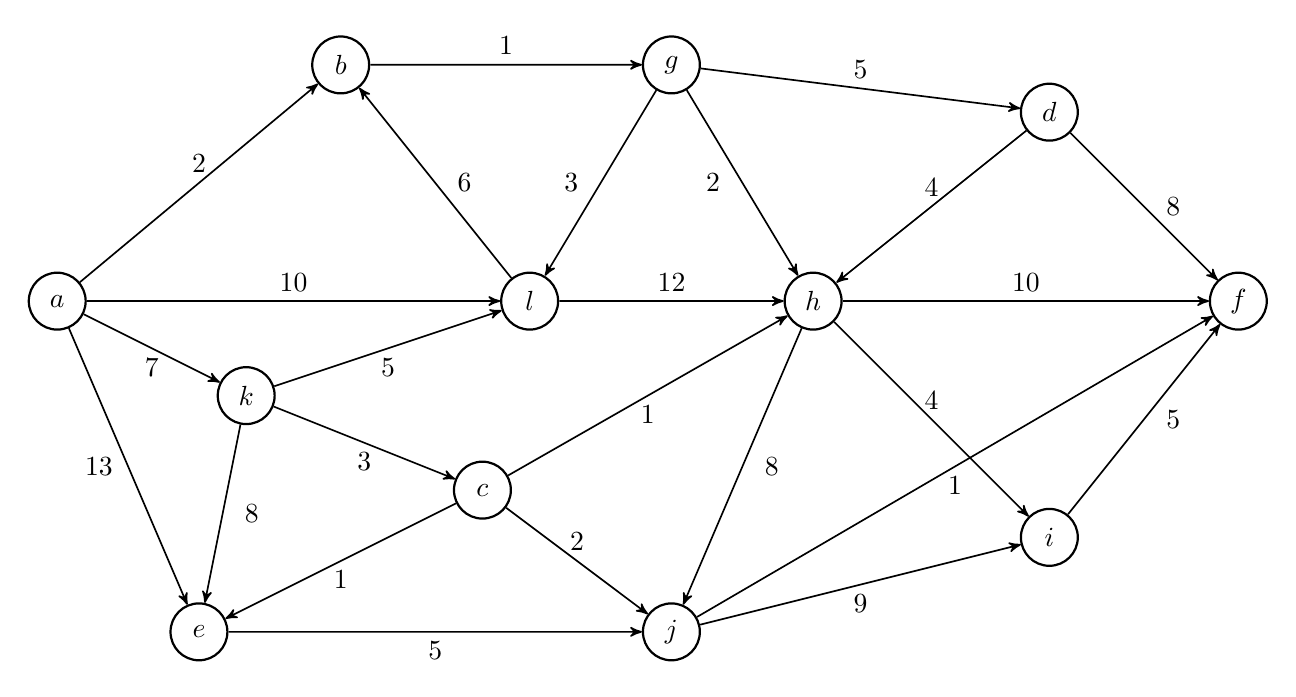
\begin{tikzpicture}
        [minimum width={width("b")+1.5em},
        vertex/.style={circle, draw=black, fill=white, thick},
        arr/.style={->,>=stealth',semithick},
        scale=1.2]
        \node (f) at (13.5, 4.5) [vertex] {$f$};
        \node (i) at (11.5, 2) [vertex] {$i$}
           edge[arr] node[right] {$5$} (f);
        \node (j) at (7.5, 1) [vertex] {$j$}
           edge[arr] node[below] {$9$} (i)
           edge[arr] node[below] {$1$} (f);
        \node (h) at (9, 4.5) [vertex] {$h$}
           edge[arr] node[above] {$10$} (f)
           edge[arr] node[above] {$4$} (i)
           edge[arr] node[right] {$8$} (j);
        \node (d) at (11.5, 6.5) [vertex] {$d$}
           edge[arr] node[right] {$8$} (f)
           edge[arr] node[above] {$4$} (h);
        \node (g) at (7.5, 7) [vertex] {$g$}
           edge[arr] node[left] {$2$} (h)
           edge[arr] node[above] {$5$} (d);
        \node (e) at (2.5, 1) [vertex] {$e$}
           edge[arr] node[below] {$5$} (j);
        \node (c) at (5.5, 2.5) [vertex] {$c$}
           edge[arr] node[below] {$1$} (e)
           edge[arr] node[above] {$2$} (j)
           edge[arr] node[below] {$1$} (h);
        \node (b) at (4, 7) [vertex] {$b$}
           edge[arr] node[above] {$1$} (g);
        \node (l) at (6, 4.5) [vertex] {$l$}
           edge[arr] node[above] {$12$} (h)
           edge[arr] node[right] {$6$} (b);
        \node (k) at (3, 3.5) [vertex] {$k$}
           edge[arr] node[below] {$3$} (c)
           edge[arr] node[right] {$8$} (e)
           edge[arr] node[below] {$5$} (l);
        \node (a) at (1, 4.5) [vertex] {$a$}
           edge[arr] node[above] {$2$} (b)
           edge[arr] node[above] {$10$} (l)
           edge[arr] node[below] {$7$} (k)
           edge[arr] node[left] {$13$} (e);
        \path (g) edge[arr] node[left] {$3$} (l);
     \end{tikzpicture}
  \end{center}
  \vspace{2\baselineskip}
\end{question}

\begin{question}
  You're in charge of a construction project. Details and duration of
  tasks of each trade are summed up in the table below. Each labeled
  task comes with the list of tasks \emph{immediatly} preceding its
  start.
    \vspace{2\baselineskip}
  \begin{center}
    \renewcommand{\arraystretch}{1.5}
    \begin{tabular}{|c|c|c|c|}
      \hline
      Label of task & Task description & Time (in weeks)  & Tasks preceding it \\
      \hline
      A  & Maconry & 12 & --   \\
      \hline
      B  & Framework & 1 & A  \\      
      \hline
      C  & Zing works & 1 & B  \\      
      \hline
      D  & Covering & 1 & C  \\      
      \hline
      E  & Electricity, first stage & 2 & D  \\      
      \hline
      F  & Sanitary facilities, first stage & 1 & D  \\      
      \hline
      G  & Glaziery & 1 & D  \\      
      \hline
      H  & Plastering & 4 & G  \\      
      \hline
      I  & Sanitary facilites, second stage & 1 & H  \\      
      \hline
      J  & Electricity, second stage & 1 & H  \\      
      \hline
      K  & Tiling & 6 & I, J  \\      
      \hline
      L  & Shutters & 1 & I  \\      
      \hline
      M  & Inside carpentry & 2 &  L \\           
      \hline
      N  & Ironmongery & 1 & L  \\      
      \hline
    \end{tabular}
  \end{center}
  \vspace{\baselineskip}
  \begin{enumerate}
  \item Draw the MPM (Meta Potential Model) graph of this project
    planning problem.
  \item Using relevant algorithms, give earliest scheduling dates. 
    \begin{itemize}
    \item What is the minimum amount of time the project needs to be done? 
    \item What are the critical tasks?
    \end{itemize}
  \item Using relevant algorithms, give latest scheduling dates.
    \begin{itemize}
    \item What is the total margin of the project? Compute free
      margins of non-critical tasks?
    \end{itemize}
  \end{enumerate}
\end{question}
\end{document}

%%% Local Variables:
%%% mode: latex
%%% TeX-master: t
%%% End:
